
\section{\texttt{gravity}}\label{sec:example_gravity}

This section presents an example of how to use QUESO in order to develop an application that solves a statistical inverse problem and
a statistical forward problem, where the solution of the former serves as input to the later. During the SIP, the acceleration due to gravity for an object in free fall near the surface of the Earth is inferred. During the SFP, the distance traveled by a projectile launched at a given angle and altitude is calculated using the calibrated magnitude of the acceleration of gravity.


In this section we describe a statistical forward problem  of predicting the  described in Section \ref{sec:gravity-ip}.

\subsection{Statistical Inverse Problem}\label{sec:gravity-ip}

% Near the surface of the Earth, an object in free fall in a vacuum will accelerate at approximately $9.8 m/s^2$, independent of its mass.
% With air resistance acting upon an object that has been dropped, mass, drag coefficient and even relative surface may become important
% (if the fall is from sufficient altitude) in the calculation of gravity.

%The vertical motion of an object falling a small distance close to the surface of the planet can be approximated to have
%uniform gravitational field without air resistance, as long as the force of gravity on the object is much greater than the force of air resistance.

%Therefore a convenient, simplified 
A possible deterministic mathematical model for the vertical motion of an object in free fall near the surface of the Earth is given by
\begin{equation}\label{eq:gravity01}
h(t)=-\frac{1}{2} g t^2 + v_0 t + h_0.
\end{equation}
where
$v_0$ [$m/s$] is the initial velocity,
$h_0$ [$m$] is the initial altitude,
$h(t)$ [$m$] is the altitude with respect to time,
$t$ [$s$] is the elapsed time, and
$g$ [$m/s^2$] is the magnitude of the acceleration due to gravity (the parameter which cannot be directly measured and will be statistically inferred).



\subsubsection{Experimental Data}
We assume that the experiment of allowing an object to fall from different altitudes with zero initial velocity has been repeatedly conducted (See Figure \ref{fig:free_fall}). The data collected, e.g.  $\mathbf{d}$, is displayed in Table \ref{table:data}; the standard deviations, $\sigma$'s, refer to the uncertainties in the measured times during the experiment execution~\cite{interactagram}. 



\begin{figure}[!ht]
\centering
\input{rawfigs/free_fall.latex}
\vspace*{-8pt}
\caption{An object falls from altitude $h_0$ with zero initial velocity ($v_0=0$).}
\label{fig:free_fall}
\end{figure}

\begin{table}[htp]%% Data from data02.dat 
\caption{Measurement data $\mathbf{d}$ of size $n_d=14$.
The object falls from altitude $h_0$ in $t$ seconds, with standard deviation of $\sigma$ seconds in the time measurement~\cite{interactagram}.
}
% \specialrule{.4pt}{10pt}{4pt}
\vspace{-8pt}
\begin{center}
\begin{tabular}{ccc}
\toprule
% $(h_0-h)$ [$m$] & $t$ [$s$]  & $\sigma$ [$s$]\\
altitude [$m$] & time [$s$]  & Std. Dev. $\sigma$ [$s$]\\
\midrule
\midrule
$~$10	&	1.41	&	0.02	\\
$~$20	&	2.14	&	0.12	\\
$~$30	&	2.49	&	0.02	\\
$~$40	&	2.87	&	0.01	\\
$~$50	&	3.22	&	0.03	\\
$~$60	&	3.49	&	0.01	\\
$~$70	&	3.81	&	0.03	\\
$~$80	&	4.07	&	0.03	\\
$~$90	&	4.32	&	0.03	\\
100	&	4.47	&	0.05	\\
110	&	4.75	&	0.01	\\
120	&	4.99	&	0.04	\\
130	&	5.16	&	0.01	\\
140	&	5.26	&	0.09	\\
\bottomrule
\end{tabular}
\end{center}
\label{table:data}
\end{table}



\subsubsection{The Prior RV, Likelihood and Posterior RV}

In a straightforward classical interpretation of Bayesian inference, the prior signifies the modeler's honest opinion about the unknown.
For the gravity inference problem, let's assume that gravity varies uniformly in the interval [8,11], or, in other words, we chose uniform prior distribution in that interval:

\begin{equation}\label{eq-g-prior}
\pi_{\text{prior}}=\mathcal{U}(8,11).
\end{equation}


We choose the usual likelihood function:
\begin{equation}\label{eq:like02}
\pi_{\text{like}}(\mathbf{d} | \boldsymbol{\theta})
\varpropto
\exp
\left\{
-\frac{1}{2}
[\mathbf{y}(\boldsymbol{\theta})-\mathbf{d}]^T
\left[\mathbf{C}(\boldsymbol{\theta})\right]^{-1}
[\mathbf{y}(\boldsymbol{\theta})-\mathbf{d}]
\right\},
\end{equation}
where $\mathbf{C}(\boldsymbol{\theta})$ is a given covariance matrix, $\mathbf{d}$ denotes experimental data, $\mathbf{y}(\boldsymbol{\theta})$ is the model output data.

Recalling the deterministic model for the acceleration of gravity (\ref{eq:gravity01}) with zero initial velocity,  the information provided in Table \ref{table:data}, and Equation (\ref{eq:like02}); and, additionally, invoking the nomenclature used in Section \ref{sec:statistical_concepts}, we have:
\begin{equation}\label{eq:like03}
\boldsymbol{\theta} \stackrel{\text{\small{def.}}}{=} g,
%------------ 
\quad
\mathbf{y}(\boldsymbol{\theta})= 
\left[
\begin{array}{c}
\sqrt{\dfrac{2 h_1}{g}}\\	
\sqrt{\dfrac{2 h_2}{g}}\\	
\vdots\\	
\sqrt{\dfrac{2 h_{n_d}}{g}}
\end{array}
\right],
%------------ 
\quad 
\mathbf{d} = 
\left[
\begin{array}{c}
t_1    \\
t_2    \\ 
\vdots \\	
t_{n_d}
\end{array}
\right],
%------------ 
\quad
\mathbf{C}(\boldsymbol{\theta})=
\left[
\begin{array}{cccc}
\sigma^2_1 & 0	        & \cdots & 0 \\
0          & \sigma^2_2 & \cdots & 0 \\
\vdots     & \vdots     & \ddots & 0 \\
0          & 0          & \cdots & \sigma^2_{n_d}
\end{array}
\right],
\end{equation}
where $n_d=14$ is the number of data points in Table \ref{table:data}.

Now we are ready to evoke Bayes' formula in order to obtain the posterior PDF $\pi_{\text{post}}(\boldsymbol{\theta})$:
\begin{equation}\label{eq-Bayes-g}
\pi_{\text{post}}(\boldsymbol{\theta}|\mathbf{d})\varpropto  \pi_{\text{like}}(\mathbf{d}|\boldsymbol{\theta}) \, \pi_{\text{prior}}(\boldsymbol{\theta}).
\end{equation}


\subsection{Statistical Forward Problem}


Projectile motion refers to the motion of an object projected into the air at an angle, e.g. a soccer ball being kicked, a baseball being thrown, or an athlete long jumping. Supposing the object does not have a propulsion system and neglecting air resistance, then the only force acting on the object is a constant gravitational acceleration $g$.


A possible deterministic two-dimensional mathematical model for the vertical motion of an object projected from near the surface of the Earth is given by
\begin{align}\label{eq:fwd01}
v_x &= v_{0x} \\ %&= v_{0} \cos(\alpha), \\
v_y &= v_{0y} - gt \\ %&= v_{0} \sin(\alpha) - gt,\\
  x &= v_{0x}t \\ %&= v_{0} \cos(\alpha) t, \\
  h &= h_0 + v_{0y}t - \frac{1}{2} g t^2  %&= v_{0} \sin(\alpha) t - \frac{1}{2} g t^2.
\end{align}
where
$h_0$ is the initial height, $x=x(t)$ is the distance traveled by the object, $\bv{v_0}=(v_{0x},v_{0y})$ is the initial velocity,
$v_{0x} = v_{0} \cos(\alpha)$, $v_{0y} = v_{0} \sin(\alpha)$, and $v_0=\|\bv{v_0}\|^2$.
%
Figure \ref{fig:projectile} displays the projectile motion of an object in these conditions.
\begin{figure}[!ht]
\centering
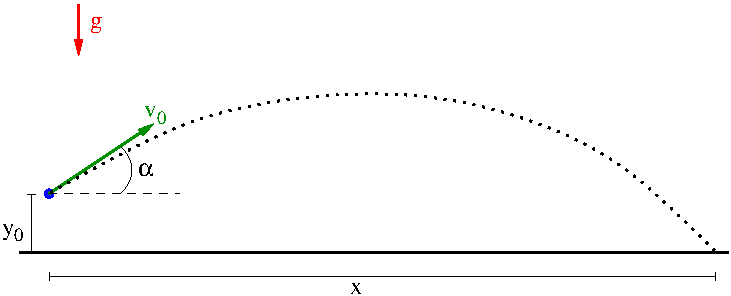
\includegraphics[scale=1]{figs/projectile}
\vspace*{-8pt}
\caption{Object traveling with projectile motion. }
\label{fig:projectile}
\end{figure}


%Assume that we want to describe the motion of such an object, starting at time $t = 0$, ... and velocity that makes an angle $\alpha$ with the $x$-axis.


For this example, we assume that $h_0 =0$ m, $\alpha = \pi/4$ radians, $v_0 = 5$ m/s, all deterministic variables; and $g$ is the solution of the SIP described in Section \ref{sec:gravity-ip}.

Since a PDF is assigned to parameter $g$; thus, the output of the mathematical model (\ref{eq:fwd01}) becomes a random variable, thus we have a statistical forward problem. 

\subsubsection{The Input RV, QoI Function and Output RV}
 
The input random variable for the statistical forward problem is the acceleration of gravity $g$, which is also the solution (posterior PDF) of the inverse problem described in Section \ref{sec:gravity-ip}. The output random variable for this example is the distance $x$ traveled by an object in projectile motion. Note that, since there is uncertainty in the parameter $g$ ($g$ is given as a PDF), one can expect that this uncertainty will be propagated to $x$, which will also be given as a PDF.

Combining the expressions in Equation \ref{eq:fwd01} and rearranging them, we have that QoI function for $x$ %(i.e. the final model for the distance traveled by an object in projectile motion) 
is: 
\begin{equation}\label{eq:fp_deterministic}
x=\dfrac{ v_0 \cos \alpha }{g} \left( v_0  \sin \alpha  + \sqrt{ ( v_0  \sin \alpha)^2 + 2g\, y_0 }\right).                                                                                        
\end{equation}
where $y$ is the distance traveled and our quantity of interest (QoI). 



\subsection{Running the Example}\label{sec:gravity-run}
 
To run the executable provided (available after QUESO installation), enter the following commands:
\begin{lstlisting}[label={},caption={}]
$ cd $HOME/LIBRARIES/QUESO-0.51.0/examples/gravity
$ rm outputData/*
$ ./gravity_gsl gravity_inv_fwd.inp
\end{lstlisting}

The console output of the program is:
\begin{lstlisting}[caption={Console output of program \texttt{gravity\_gsl}}, label={code:console_output},language={bash}]
kemelli@violeta:~/LIBRARIES/QUESO-0.51.0/examples/gravity$ ./gravity_gsl gravity_inv_fwd.inp 
---------------------------------------------------------------------
QUESO Library: Version = 0.47.1 (47.1)

Development Build

Build Date   = 2013-04-29 17:05
Build Host   = violeta
Build User   = kemelli
Build Arch   = x86_64-unknown-linux-gnu
Build Rev    = 38998M

C++ Config   = mpic++ -g -O2 -Wall

Trilinos DIR = 
GSL Libs     = -L/home/kemelli/LIBRARIES/gsl-1.15/lib -lgsl -lgslcblas -lm
GRVY DIR     = 
GLPK DIR     = 
HDF5 DIR     = /home/kemelli/LIBRARIES/hdf5-1.8.10
--------------------------------------------------------------------------------------------------------------
Beginning run at Mon Apr 29 17:27:32 2013

MPI node of worldRank 0 has fullRank 0, belongs to subEnvironment of id 0, and has subRank 0
MPI node of worldRank 0 belongs to sub communicator with full ranks 0
MPI node of worldRank 0 also belongs to inter0 communicator with full ranks 0, and has inter0Rank 0


Beginning run of 'Gravity + Projectile motion' example at Mon Apr 29 17:27:32 2013

 my fullRank = 0
 my subEnvironmentId = 0
 my subRank = 0
 my interRank = 0

Beginning 'SIP -> Gravity estimation' at Mon Apr 29 17:27:32 2013

Solving the SIP with Metropolis Hastings

Beginning 'SFP -> Projectile motion' at Mon Apr 29 17:27:33 2013

Solving the SFP with Monte Carlo

Ending run of 'Gravity + Projectile motion' example at Mon Apr 29 17:27:33 2013

Ending run at Mon Apr 29 17:27:33 2013
Total run time = 1 seconds
kemelli@violeta:~/LIBRARIES/QUESO-0.51.0/examples/gravity$ 
\end{lstlisting}


In order to generate chain plots, histograms, KDEs, etc., the user may use Matlab/GNU Octave and call the following command lines:
\begin{lstlisting}
$ matlab
   $ gravity_plots_ip      # inside matlab
   $ gravity_plots_fp      # inside matlab
   $ exit                  # inside matlab
$ ls -l outputData/*.png
  sfp_gravity_autocorrelation.png  sfp_gravity_cdf.png
  sfp_gravity_chain_pos.png        sfp_gravity_hist.png
  sfp_gravity_kde.png              sip_gravity_autocorrelation_raw_filt.png
  sip_gravity_cdf_filt.png         sip_gravity_cdf_raw.png
  sip_gravity_chain_pos_filt.png   sip_gravity_chain_pos_raw.png
  sip_gravity_hist_filt.png        sip_gravity_hist_raw.png
  sip_gravity_kde_filt.png         sip_gravity_kde_raw.png
\end{lstlisting}

As a result, the user should have created several of PNG figures containing marginal posterior PDF, chain positions of the parameters and the QoI, histogram, cumulative density distribution and autocorrelation. The name of the figure files have been chosen to be informative, as shown in the Listing above.



\subsection{Example Code}\label{sec:gravity_code}

The source code for the SIP and the SFP is composed of 7 files.
Three of them are common for both problems: \texttt{gravity\_main.C, gravity\_compute.h} and \texttt{gravity\_compute.C}; they combine both problems and use the solution of the SIP (the posterior PDF for the gravity) as an input for the SFP and are presented, respectively, in Listings \ref{code:gravity_main}, \ref{code:gravity_compute_h} and \ref{code:gravity_compute_C}.
Two of files specifically  handle the SIP: \texttt{gravity\_likelihood.h}, and \texttt{gravity\_likelihood.C}, and are displayed in Listings \ref{code:gravity_like_h} and \ref{code:gravity_like_C}. Finally, the files specific for the SFP are \texttt{gravity\_qoi.h} and \texttt{gravity\_qoi.C}, and they are presented in Listings \ref{code:gravity_qoi_h} and \ref{code:gravity_qoi_C}.

\lstinputlisting[caption=File \texttt{gravity\_main.C.}, label=code:gravity_main, linerange={25-1000}]{../../examples/gravity/src/gravity_main.C}
 
\lstinputlisting[caption=File \texttt{gravity\_compute.h.}, label=code:gravity_compute_h, linerange={32-1000}]{../../examples/gravity/src/gravity_compute.h}

\lstinputlisting[caption={File \texttt{gravity\_compute.C}. The first part of the code (lines 60--150) handles the statistical forward problem, whereas the second part of the code (lines 151--216) handles the statistical forward problem.\\}, label=code:gravity_compute_C, linerange={26-1000},numbers=left]{../../examples/gravity/src/gravity_compute.C}

\lstinputlisting[caption=File \texttt{gravity\_likelihood.h}., label=code:gravity_like_h, linerange={32-1000}]{../../examples/gravity/src/gravity_likelihood.h}

\lstinputlisting[caption=File \texttt{gravity\_likelihood.C}., label=code:gravity_like_C, linerange={31-1000}]{../../examples/gravity/src/gravity_likelihood.C}

\lstinputlisting[caption=File \texttt{gravity\_qoi.h}., label=code:gravity_qoi_h, linerange={32-1000}]{../../examples/gravity/src/gravity_qoi.h}

\lstinputlisting[caption=File \texttt{gravity\_qoi.C}., label=code:gravity_qoi_C, linerange={32-96}]{../../examples/gravity/src/gravity_qoi.C}

\subsection{Input File}\label{sec:gravity-input-file}

QUESO reads an input file for solving statistical problems.
In the case of a SIP, it expects a list of options for MCMC, while in case of SFP it expects a list of options for Monte Carlo. The  input file `\texttt{gravity\_inv\_fwd.inp} used in this example is presented in Listing \ref{code:gravity_inv_fwd}.

\lstinputlisting[caption=Some options for QUESO library used in application code (Listings \ref{code:gravity_main}-\ref{code:gravity_like_C})., label={code:gravity_inv_fwd},]{../../examples/gravity/tests/test_2013_01_22/gravity_inv_fwd.inp}


 

Moreover, for the gravity inverse problem, one may notice that QUESO will use the Metropolis-Hastings algorithm to sample the posterior PDF
(indicated by the prefix \texttt{mh\_}in the variable names) without adaptive steps
(indicated by the zero value assigned to the variable \linebreak \texttt{ip\_mh\_am\_initialNonAdaptInterval}, which can also be achieved by setting zero to \linebreak
\verb+ip_mh_am_adaptInterval+) and with delayed rejection (indicated by the one-value assigned to the variable \texttt{ip\_mh\_dr\_maxNumExtraStages}).



 
\subsection{Create your own Makefile}\label{sec:gravity-makefile}



Listing \ref{code:makefile} presents a Makefile, named \texttt{Makefile\_example\_violeta}, that may be used to compile the code and create the executable \verb+gravity_gsl+. Naturally, it must be adapted to the user's settings, i.e., it has to have the correct paths for the user's libraries that were actually used to compile and install QUESO (see Sections \ref{sec:Pre_Queso}--\ref{sec:install_Queso_make}).

\lstinputlisting[caption={Makefile for the application code in Listings \ref{code:gravity_main}-\ref{code:gravity_like_C}},  label={code:makefile},language={bash}]{../../examples/gravity/src/Makefile_example_violeta}




\subsection{Running the Gravity Example with Several Processors}

Even though the application described in Section \ref{sec:gravity_code} is a serial code, it is possible to run it using more than one processor, i.e., in parallel mode. 
Supposing the user's workstation has $N_p=8$ processors, then, the user my choose to have $N_s =$ 8, 4 or 2 subenvironments. This complies with the requirement that the total number of processors in the environment must be a multiple of the specified number of subenvironments.

Thus, to build and run the application code with $N_p = 8$, and $N_s=8$ subenvironments, the must set the variable \texttt{env\_numSubEnvironments = 8} in the input file (Listing~\ref{code:gravity_inv_fwd}) and enter the following command lines: 



\begin{lstlisting}[caption={}, label={},language={bash}]
cd $HOME/LIBRARIES/QUESO-0.51.0/examples/gravity/
mpirun -np 8 ./gravity_gsl gravity_inv_fwd.inp
\end{lstlisting}


The steps above will create a total number of 8 raw chains, of size defined by the variable \texttt{ip\_mh\_rawChain\_size}. QUESO internally combines these 8 chains into a single chain of size $8\; \times\,$\texttt{ip\_mh\_rawChain\_size} and saves it in a file named according to the variable \texttt{ip\_mh\_rawChain\_dataOutputFileName}. 
QUESO also provides the user with the option of writing each chain -- handled by its corresponding processor -- in a separate file, which is accomplished by setting the variable \texttt{ip\_mh\_rawChain\_dataOutputAllowedSet = 0 1 ... Ns-1}.\\

\noindent
{\bf Note:} Although the discussion in the previous paragraph refers to the raw chain of a SIP, the analogous is true for the filtered chains (SIP), and for the samples employed in the SFP (\texttt{ip\_mh\_filteredChain\_size},    \texttt{fp\_mc\_qseq\_size} and \texttt{fp\_mc\_qseq\_size}, respectively). 




\subsection{Data Post-Processing and Visualization}\label{sec:gravity-results}

 

According to the specifications of the input file in Listing~\ref{code:gravity_inv_fwd}, both a folder named \verb+outputData+ and a the following files should be generated:
\begin{verbatim}
sfp_gravity_sub0.m,         sip_gravity_sub0.m, 
sfp_gravity_p_seq.m,        sip_gravity_filtered_chain.m,,
sfp_gravity_p_seq_sub0.m    sip_gravity_filtered_chain_sub0.m,
sfp_gravity_qoi_seq.m,      sip_gravity_raw_chain.m,       
sfp_gravity_qoi_seq_sub0.m  sip_gravity_raw_chain_sub0.m,
display_env_sub0.txt 
\end{verbatim}

%The names of the files have been chosen to be informative.


%In this case, only one sub-environment (processor) has been used, thus, only one file of the type \verb+display_env_sub*+ is generated.
%

In this section, a convenient capability of QUESO of internally handling possible conflicts in chain size is presented. Recalling the input file \verb+gravity_inv_fwd.inp+ presented in Listing~\ref{code:gravity_inv_fwd}, one may notice that  the raw chain size for the SIP is chosen to have 20000 positions (\verb+ip_mh_rawChain_size = 20000+); the lag of the filtered chain is chosen to be 20 (\verb+ip_mh_filteredChain_lag = 20+) and the chain size for the SFP has 16384 positions (\verb+fp_mc_qseq_size = 16384+). Because the solution of the SIP, ie, the posterior PDF, is used as input PDF for the SFP, QUESO internally sets \verb+fp_mc_qseq_size = 20000+, as can be seen in the file \verb+display_env_sub0.txt+.  The file \verb+display_env_sub0.txt+ contains information from the subenvironment `0' that was generated during the run of the application code.

\subsubsection{Statistical Inverse Problem}

There are a few Matlab-ready commands that are very helpful tools for post-processing the data generated by QUESO when solving statistical inverse problems.
This section discusses the results computed by QUESO with the code of Section \ref{sec:gravity_code}, and shows how to use Matlab for the post-processing of such results.

\paragraph{Chain Plots}\

It is quite simple to plot, using Matlab, the chain of positions used in the DRAM algorithm implemented within QUESO. 
The sequence of Matlab commands presented in Listing \ref{matlab:chain} generates the graphic depicted in Figure \ref{fig:sip_gravity_chain_pos_raw}.
Figure~\ref{fig:sip_gravity_chain_pos_filtered} is obtained analogously. % by loading \verb+sip_gravity_filtered_chain+ and using  \verb+ip_mh_filtChain_unified+ inside \verb+plot+.

\begin{lstlisting}[label=matlab:chain,caption={Matlab code for the chain plot.}]
% inside Matlab
>> sip_gravity_raw_chain
>> plot(ip_mh_rawChain_unified)
>> ylabel('\theta=g','fontsize',20);
>> xlabel('Number of positions','fontsize',20);
>> title('DRAM Chain Positions (raw)','fontsize',20);
\end{lstlisting}

\begin{figure}[p]
\centering 
\subfloat[Raw chain]{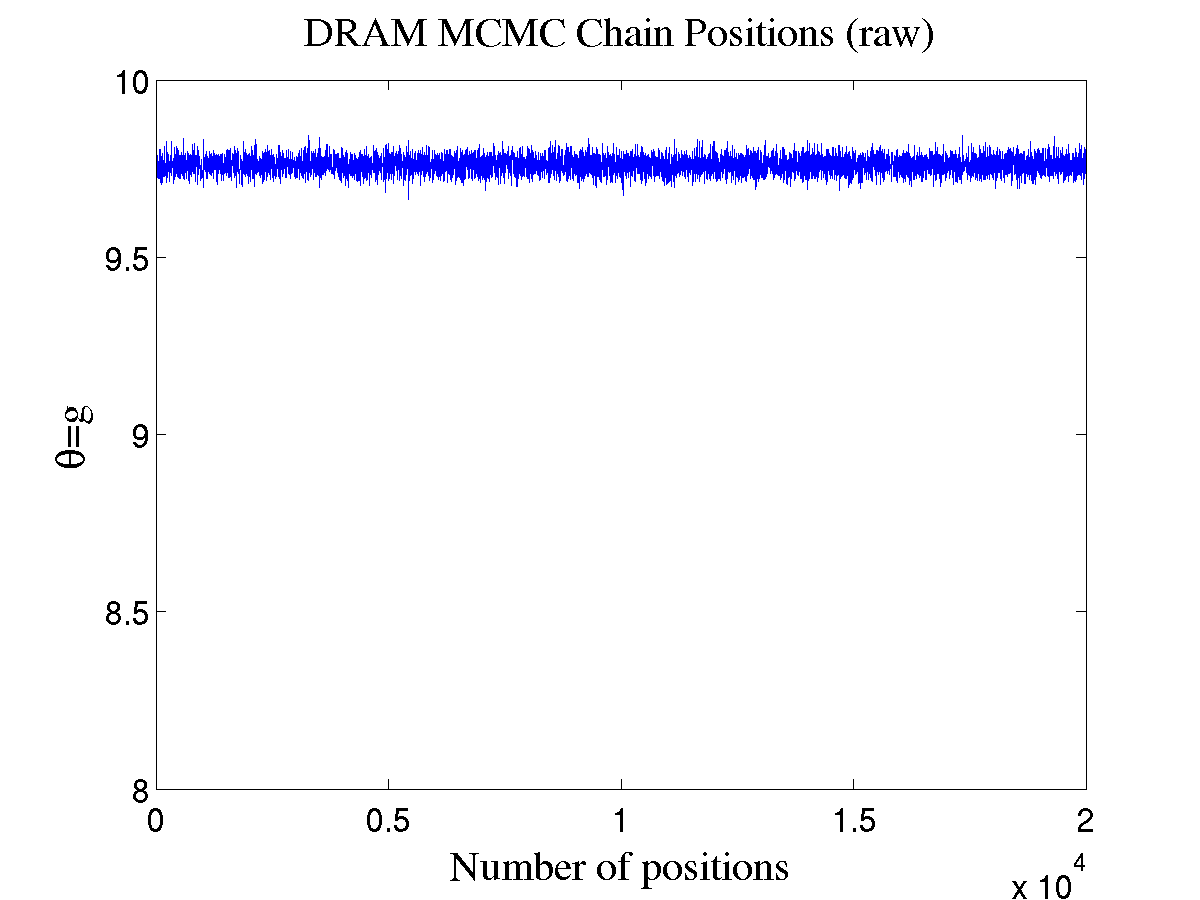
\includegraphics[scale=0.35]{figs/sip_gravity_chain_pos_raw.png}\label{fig:sip_gravity_chain_pos_raw}}
\subfloat[Filtered chain]{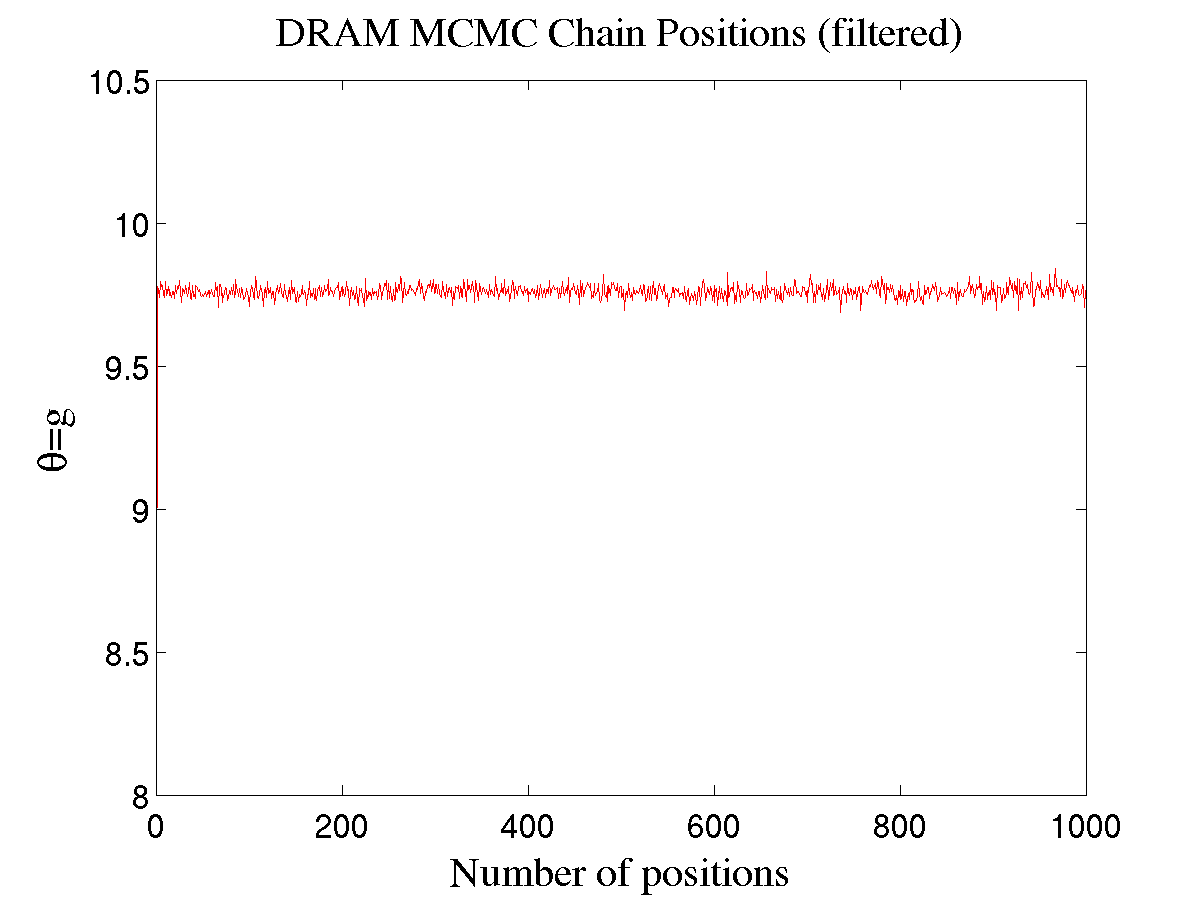
\includegraphics[scale=0.35]{figs/sip_gravity_chain_pos_filt.png}\label{fig:sip_gravity_chain_pos_filtered}}
\vspace*{-10pt}
\caption{MCMC raw chain with \chainsizeresults{} positions and a filtered chain with lag of 20 positions.}
\end{figure}

\paragraph{Histogram Plots}\

In order to plot histograms of the parameter using either the raw chain or the filtered chain, you simply have to use the pre-defined Matlab function \verb+hist+.
%The Matlab code presented in Listing \ref{matlab:hist} below shows how to create the Figure \ref{fig:sip_gravity_hist_raw};
%once more, Figure \ref{fig:sip_gravity_hist_filtered} is obtained by making suitable adjustments on that code.
%
\begin{lstlisting}[label=matlab:hist,caption={Matlab code for the histogram plot.}]
% inside Matlab
>> sip_gravity_raw_chain
>> nbins=100;
>> hist(ip_mh_rawChain_unified,nbins)
>> title('Parameter Histogram (raw chain)','fontsize',20);
>> xlabel('Gravity (m/s^2)','fontsize',20);
>> ylabel('Frequency','fontsize',20);
>> grid on;
\end{lstlisting}

\begin{figure}[p]
\centering 
\subfloat[Raw chain]{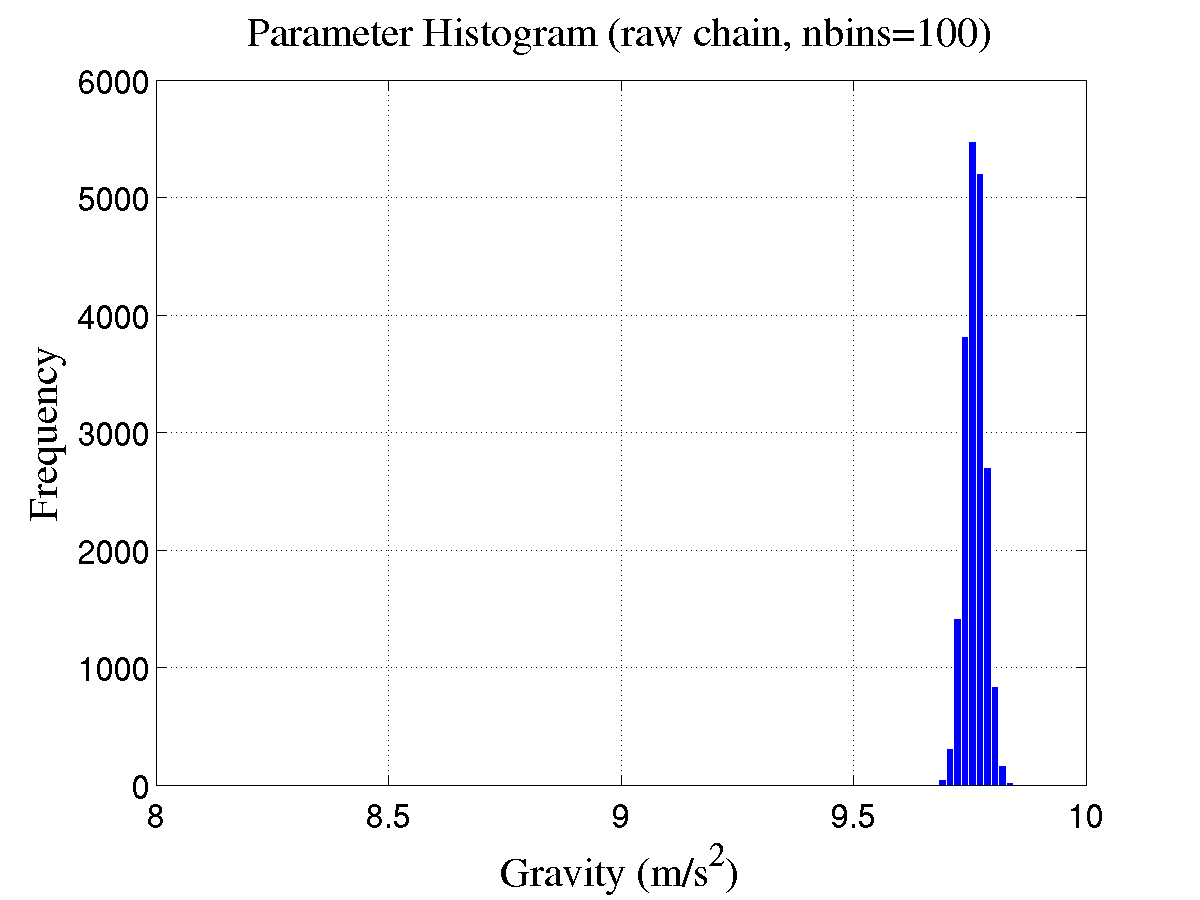
\includegraphics[scale=0.35]{figs/sip_gravity_hist_raw.png}\label{fig:sip_gravity_hist_raw}}
\subfloat[Filtered chain]{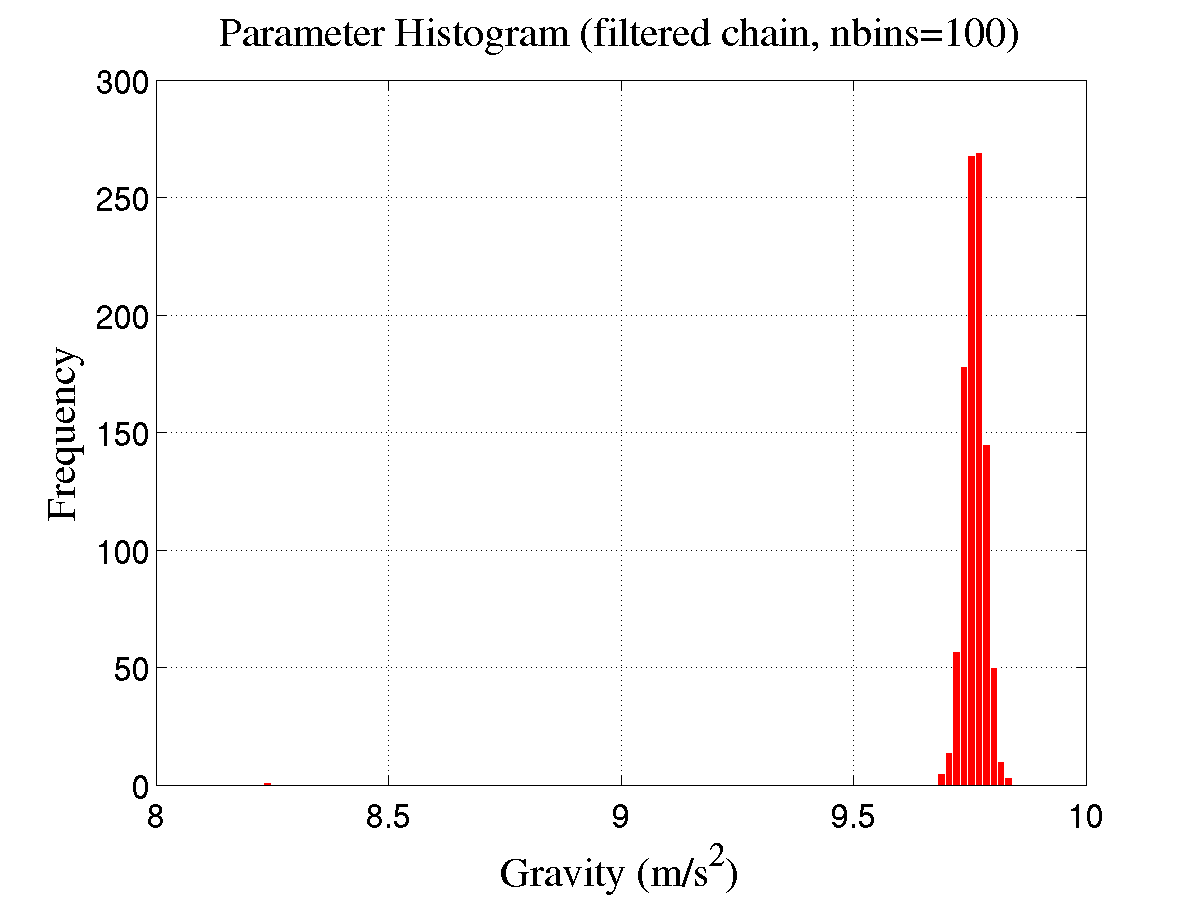
\includegraphics[scale=0.35]{figs/sip_gravity_hist_filt.png}\label{fig:sip_gravity_hist_filtered}}
\vspace*{-10pt}
\caption{Histograms of parameter $\theta=g$. }
\end{figure}

\paragraph{KDE Plots} \

Matlab function \verb+ksdensity+ (Kernel smoothing density estimate) together with the option \verb+'pdf'+ may be used for plotting the KDE of the parameter.
\begin{lstlisting}[label=matlab:kde,caption={Matlab code for the KDE plot.}]
% inside Matlab
>> sip_gravity_raw_chain
>> [f,xi] = ksdensity(ip_mh_rawChain_unified,'function','pdf');
>> plot(xi,f,'-b','linewidth',3)
>> title('Parameter Kernel Density Estimation','fontsize',20);
>> xlabel('Gravity (m/s^2)','fontsize',20);
>> ylabel('KDE','fontsize',20);
>> grid on;
\end{lstlisting}

%Figure \ref{fig:sip_gravity_kde_raw} is created by using Matlab commands presented in Listing \ref{matlab:kde} above.
\begin{figure}[p]
\centering 
\subfloat[Raw chain]{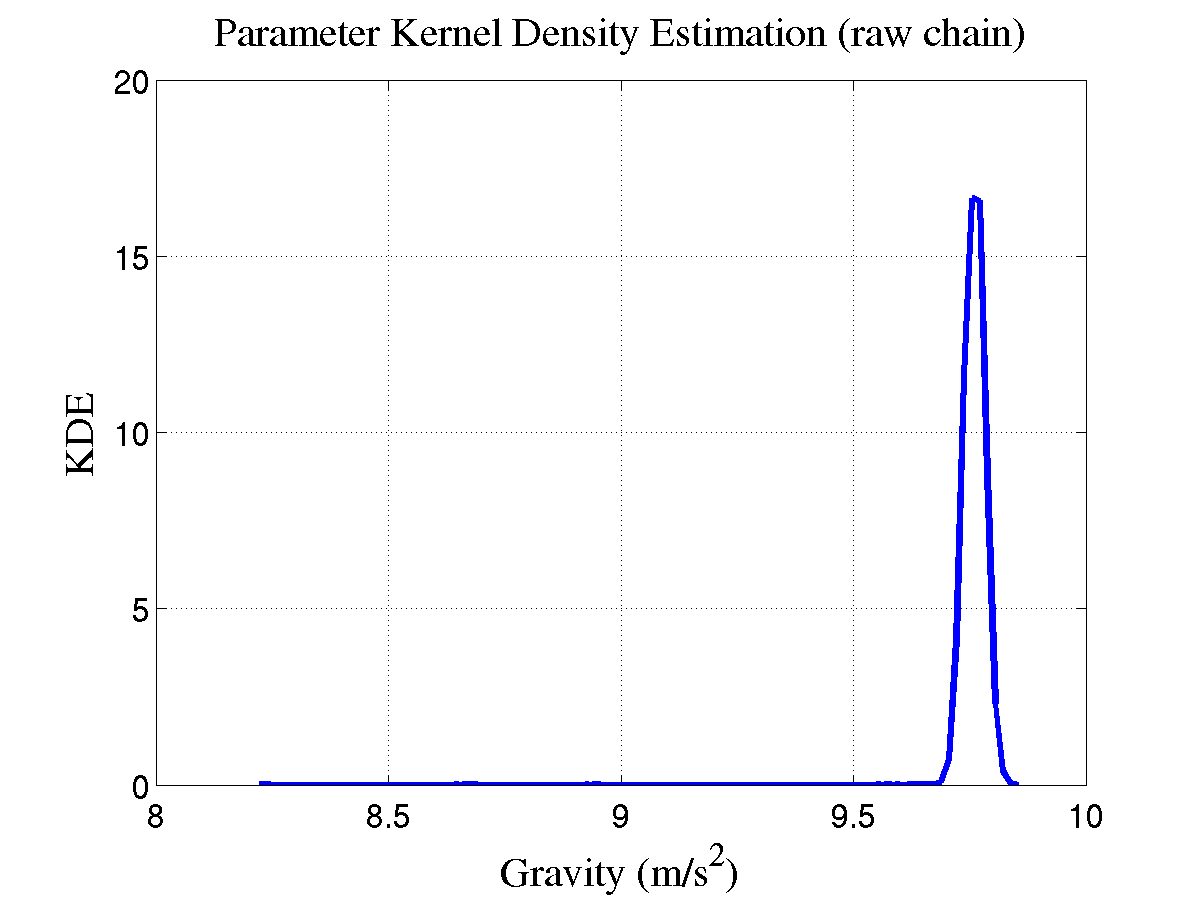
\includegraphics[scale=0.35]{figs/sip_gravity_kde_raw.png}\label{fig:sip_gravity_kde_raw}}
\subfloat[Filtered chain]{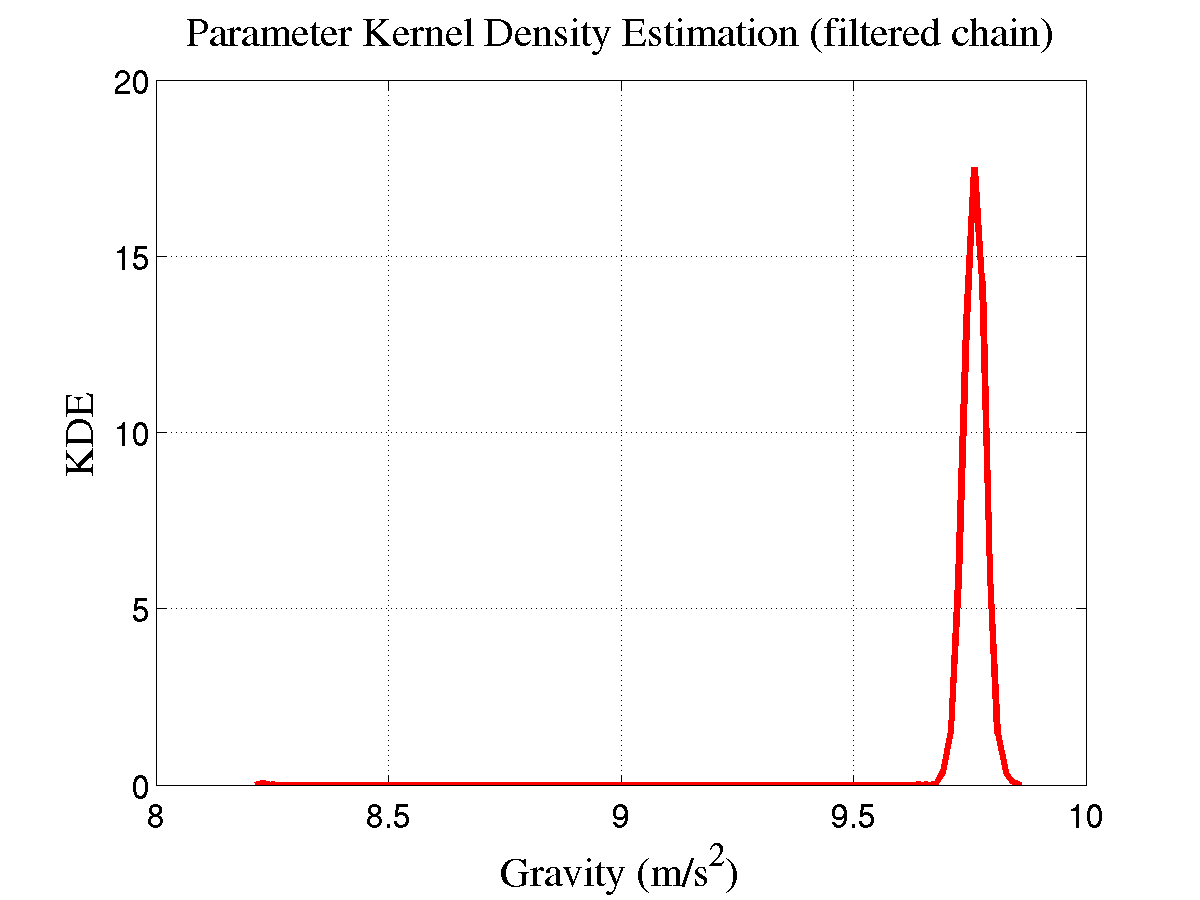
\includegraphics[scale=0.35]{figs/sip_gravity_kde_filt.png}\label{fig:sip_gravity_kde_filtered}}
\vspace*{-10pt}
\caption{Kernel Density Estimation. }
\end{figure}


% \subsubsection{Checking a KDE Plot Against Brute-Force Plot of the Likelihood Function}
% 
% See Figure \ref{fig:sip_gravity_compare_brute_force_unnormal}.
% %Figures \ref{fig:sip_gravity_compare_brute_force_unnormal} and \ref{fig:sip_gravity_compare_brute_force_normal} depict unnormalized and normalized KDE distributions
% %comparing the solution of the SIP provided by QUESO ($\pi_{\text{post}} (g)$) and the analytical (brute force) distribution.
% 
% \begin{figure}[htpb]
% \centering 
% %\subfloat[Unnormalized]{\includegraphics[scale=0.35]{figs/gravity_likelihood_brute_force_compare_post_pdf_0.png}\label{fig:sip_gravity_compare_brute_force_unnormal}}
% %\subfloat[Normalized]{\includegraphics[scale=0.35]{figs/gravity_likelihood_brute_force_compare_post_pdf_normalized0.png}\label{fig:sip_gravity_compare_brute_force_normal}}
% \subfloat{\includegraphics[scale=0.35]{figs/gravity_likelihood_brute_force_compare_post_pdf_0.png}\label{fig:sip_gravity_compare_brute_force_unnormal}}
% \vspace*{-10pt}
% \caption{Comparison of the posterior KDE for $g$ against the brute force calculation of the likelihood on a regular grid on $g$.
% }
% \end{figure}
% 
% %The code had to be slightly modified in order to replace QUESO sampling from the uniform distribution for the gravity with what we call a `brute force sampling'.
% %This brute force `sampling'  consists of recovering a pre-defined amount of values for $g$ from an equally spaced interval.
% %This is accomplished in lines 75 -- 100 of code \ref{code:gravity_compute_bruteforce_C}: it replaces Steps 4-6 (lines 100-150)
% %of the original application code provided in Algorithm \ref{code:gravity_compute_C}.
% 
% %\lstinputlisting[caption={Application code modified to `brute force' sampling from pre-defined interval.}, label={code:gravity_compute_bruteforce_C},  linerange={28-1000}]{../../brute_force/gravity_compute.C}
%  
% %Once more, Matlab function \verb+ksdensity+ (Kernel smoothing density estimate) may be used for plotting the KDE of the parameter.
% %The Matlab code below is responsible for the generation of Figure \ref{fig:sip_gravity_compare_brute_force_unnormal}.
% %Note that it reads the file \verb+gravity_likeli_brute_force.dat+, which is an output of the brute force code depicted in Listing \ref{code:gravity_compute_bruteforce_C}.
% %%
% %\begin{lstlisting}[label=matlab:kde_bruteforce,caption={Matlab code for the comparison of KDE plot from QUESO and `brute force'.}]
% %% inside Matlab
% %>> [g,like]=textread('gravity_likeli_brute_force.dat', '%f %f' );
% %>> [f,xi] = ksdensity(ip_mh_rawChain_unified,'function','pdf');
% %>> [haxes,hline1,hline2] = plotyy(xi,f,g,exp(like),'plot', 'plot');
% %>> axes(haxes(1));
% %>> ylabel('\pi_{post}(g) - QUESO/raw chain','fontname', 'Times', 'fontsize',20);
% %>> axes(haxes(2));
% %>> ylabel('\pi_{like}(g) -  brute force','fontname', 'Times', 'fontsize',20);
% %>> grid on;
% %>> title('Unnormalized distributions','fontname', 'Times', 'fontsize',20);
% %>> set(hline1,'linewidth',3);
% %>> set(hline2,'linewidth',3);
% %\end{lstlisting}


\paragraph{CDF Plots} \

Matlab function \verb+ksdensity+ (Kernel smoothing density estimate) with \verb+'cdf'+ option may also be used for plotting the Cumulative Distribution Function of the parameter.


\begin{lstlisting}[label=matlab:cdf,caption={Matlab code for the CDF plot.}]
% inside Matlab
>> sip_gravity_raw_chain
>> [f,xi] = ksdensity(ip_mh_rawChain_unified,'function','cdf');
>> plot(xi,f,'-b','linewidth',3)
>> title('Parameter Cumulative Distribution Function','fontsize',20);
>> xlabel('Gravity (m/s^2)','fontsize',20);
>> ylabel('CDF','fontsize',20);
>> grid on;
\end{lstlisting}

%Similarly, Figure \ref{fig:sip_gravity_cdf_raw} is created by using above Matlab commands.
\begin{figure}[p]
\centering 
\subfloat[Raw chain]{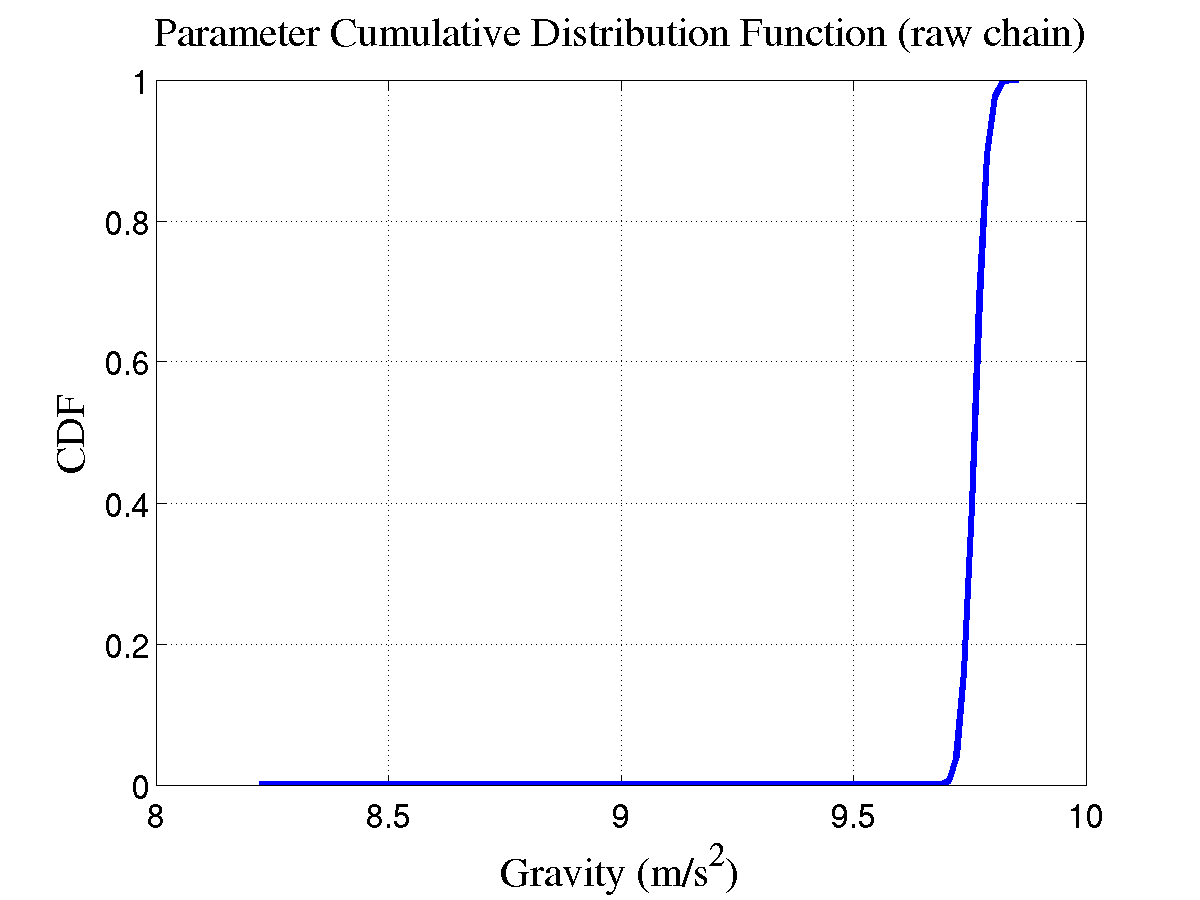
\includegraphics[scale=0.35]{figs/sip_gravity_cdf_raw.png}\label{fig:sip_gravity_cdf_raw}}
\subfloat[Filtered chain]{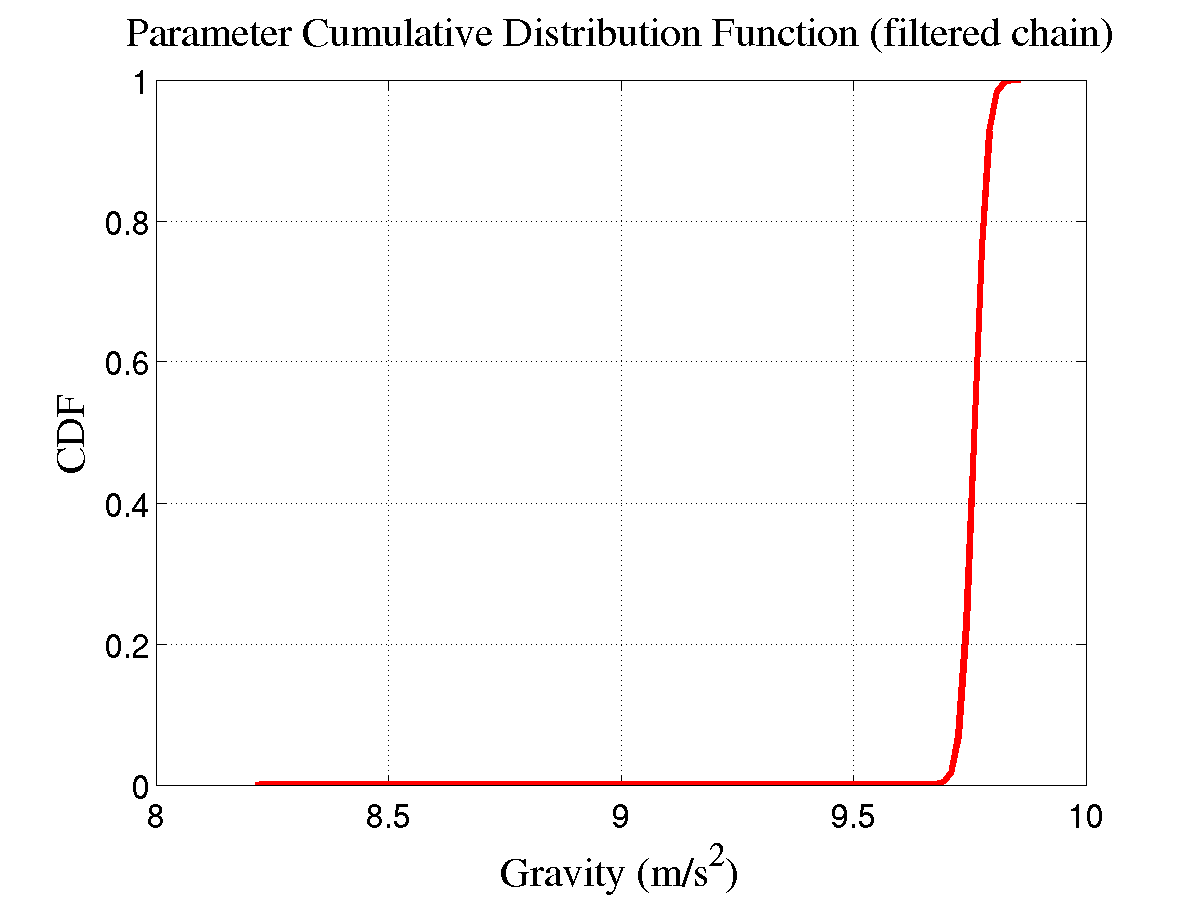
\includegraphics[scale=0.35]{figs/sip_gravity_cdf_filt.png}\label{fig:sip_gravity_cdf_filtered}}
\vspace*{-10pt}
\caption{Cumulative Distribution Function. }
\end{figure}

\paragraph{Autocorrelation Plots}\

The code presented in Listing \ref{matlab:autocorr} uses matlab function \verb+autocorr+ to generate Figure \ref{fig:sip_gravity_autocorrelation_raw_filt}
which presents the autocorrelation of the parameter $g$ in both cases: raw and filtered chain.

\begin{lstlisting}[label=matlab:autocorr,caption={Matlab code for the autocorrelation plots.}]
% inside Matlab
>> sip_gravity_raw_chain
>> sip_gravity_filtered_chain
>> nlags=10;
>> [ACF_raw,lags,bounds]= autocorr(ip_mh_rawChain_unified, nlags, 0);
>> [ACF_filt,lags,bounds]=autocorr(ip_mh_filtChain_unified,nlags, 0);
>> plot(lags,ACF_raw,'bo-',lags,ACF_filt,'r*-','linewidth',3);
>> ylabel('Autocorrelation for \theta=g','fontsize',20);
>> xlabel('Lag','fontsize',20);
>> title('Parameter Autocorrelation','fontsize',20);
>> grid on;
>> h=legend('raw chain','filtered chain','location','northeast');
>> set(h,'fontsize',16);
\end{lstlisting}

\begin{figure}[p]
\centering
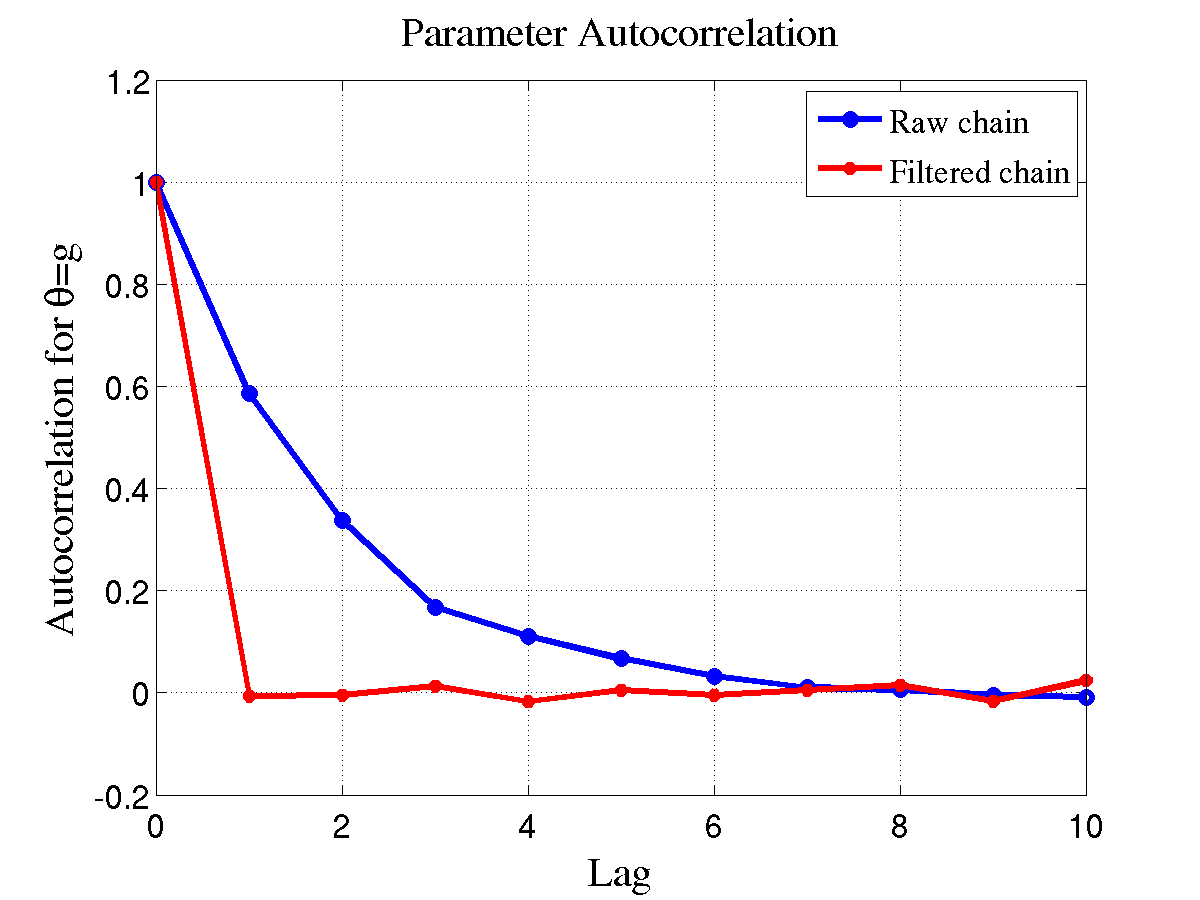
\includegraphics[scale=0.35]{figs/sip_gravity_autocorrelation_raw_filt.png}
\vspace{-8pt}
\caption{
Autocorrelation plots. }
\label{fig:sip_gravity_autocorrelation_raw_filt}
\end{figure}

\paragraph{Covariance and Correlation Matrices}\

Matlab function \verb+cov+ calculates the covariance matrix for a data matrix (where each column represents a separate quantity), and \verb+corr+ calculates the correlation matrix.
Since our statistical inverse problem has only one parameter (the acceleration $g$ due to gravity), both covariance and correlation matrices have dimension $1 \times 1$, i.e., they are scalars.

\begin{lstlisting}[label=matlab:cov_matrix,caption={Matlab code for finding the covariance matrix.}]
% inside Matlab
>> sip_gravity_raw_chain;
>> cov_matrix_g = cov(ip_mh_rawChain_unified)
   
cov_matrix_g =

   6.8709e-04
>> corr_matrix_g = corr(ip_mh_rawChain_unified)

corr_matrix_g =

     1
>>
\end{lstlisting}

\newpage

\subsubsection{Statistical Forward Problem}


\paragraph{Chain Plots} \

It is quite simple to plot, using Matlab, the chain of positions generated by the Monte Carlo algorithm implemented within QUESO and called during the solution of the statistical forward problem. 
The sequence of Matlab commands presented bellow generates the graphic depicted in Figure~\ref{fig:sfp_gravity_chain}. 

\begin{lstlisting}[label=matlab:chain_qoi,caption={Matlab code for the chain plot.}]
% inside Matlab
>> sfp_gravity_qoi_seq.m
>> plot(fp_mc_QoiSeq_unified);
>> ylabel('QoI','fontsize',20);
>> xlabel('Number of positions','fontsize',20);
>> title('MC Chain Positions','fontsize',20);
\end{lstlisting}

% \begin{figure}[p]
% \centering 
% 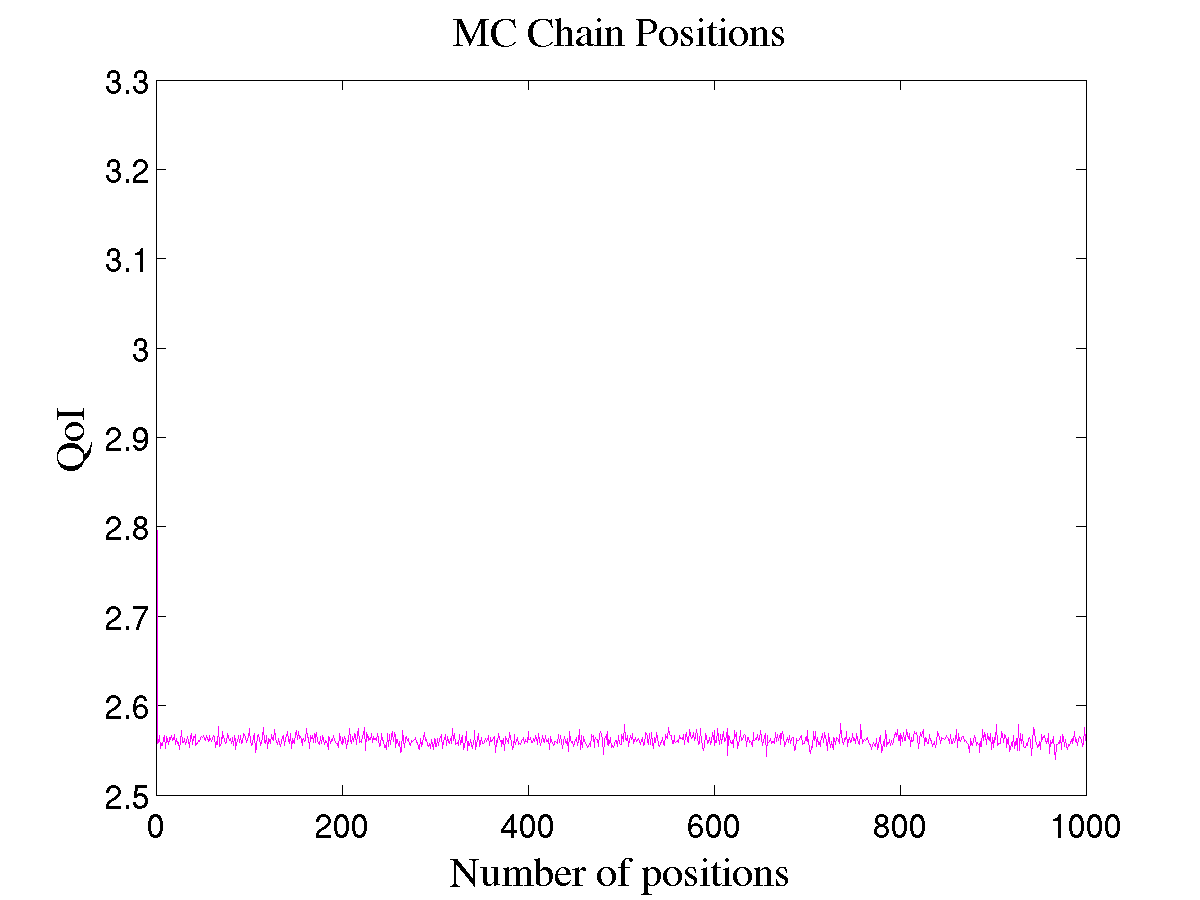
\includegraphics[scale=0.35]{figs/sfp_gravity_chain_pos.png}
% \vspace*{-10pt}
% \caption{MC chain positions for the QoI.}
% \label{fig:sfp_gravity_chain}
% \end{figure}

\paragraph{Histogram Plots} \

In order to plot a histogram of the QoI, you may use the pre-defined Matlab function \verb+hist+.
The Matlab code presented in below shows how to create the Figure~\ref{fig:sfp_gravity_hist}.

\begin{lstlisting}[label=matlab:hist_qoi,caption={Matlab code for the QoI histogram plot.}]
>> sfp_gravity_qoi_seq.m
>> nbins=100;
>> hist(fp_mc_QoiSeq_unified);
>> title('QoI Histogram','fontsize',20);
>> xlabel('Distance traveled (m)','fontsize',20);
>> ylabel('Frequency','fontsize',20);
>> grid on;
\end{lstlisting}

\begin{figure}[h]
\centering 
\subfloat[Chain positions]{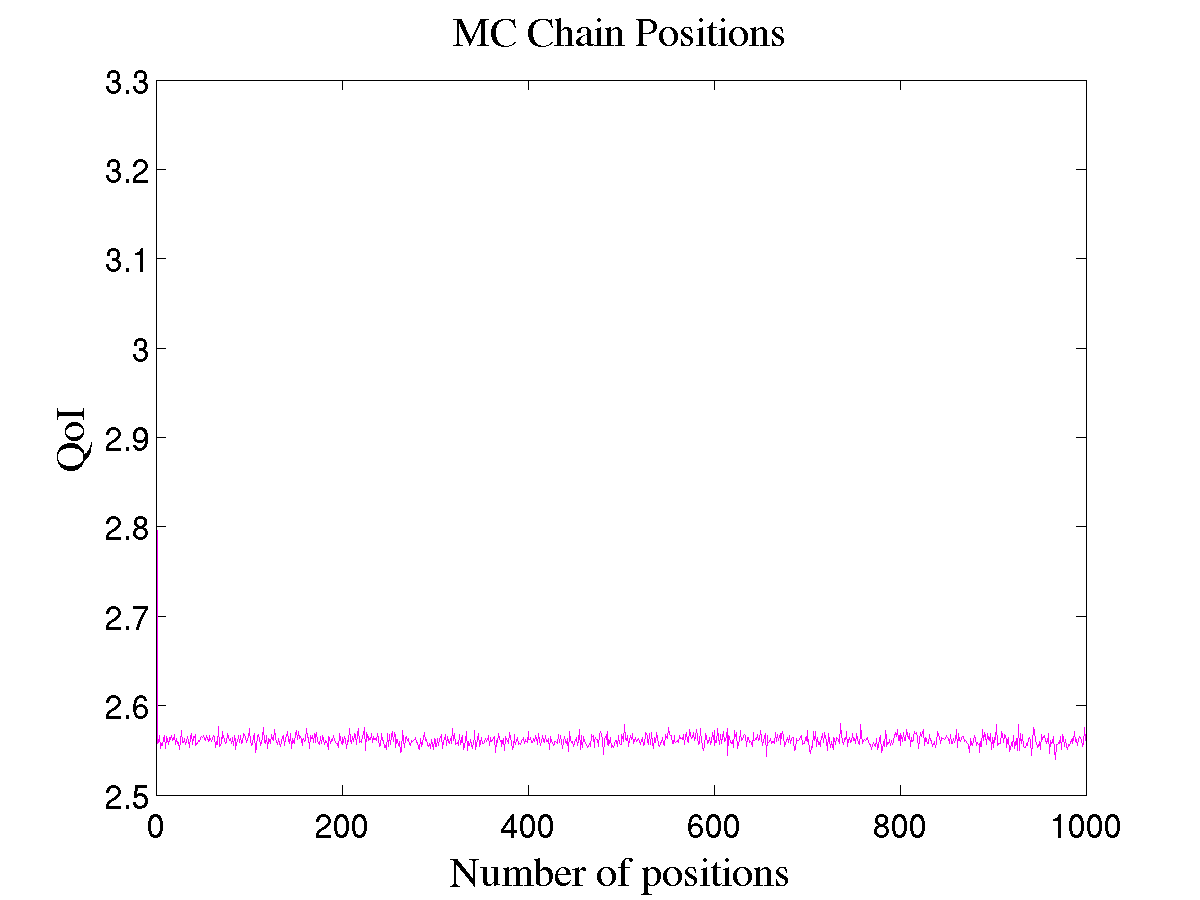
\includegraphics[scale=0.35]{figs/sfp_gravity_chain_pos.png}\label{fig:sfp_gravity_chain}}
\subfloat[Hystogram]{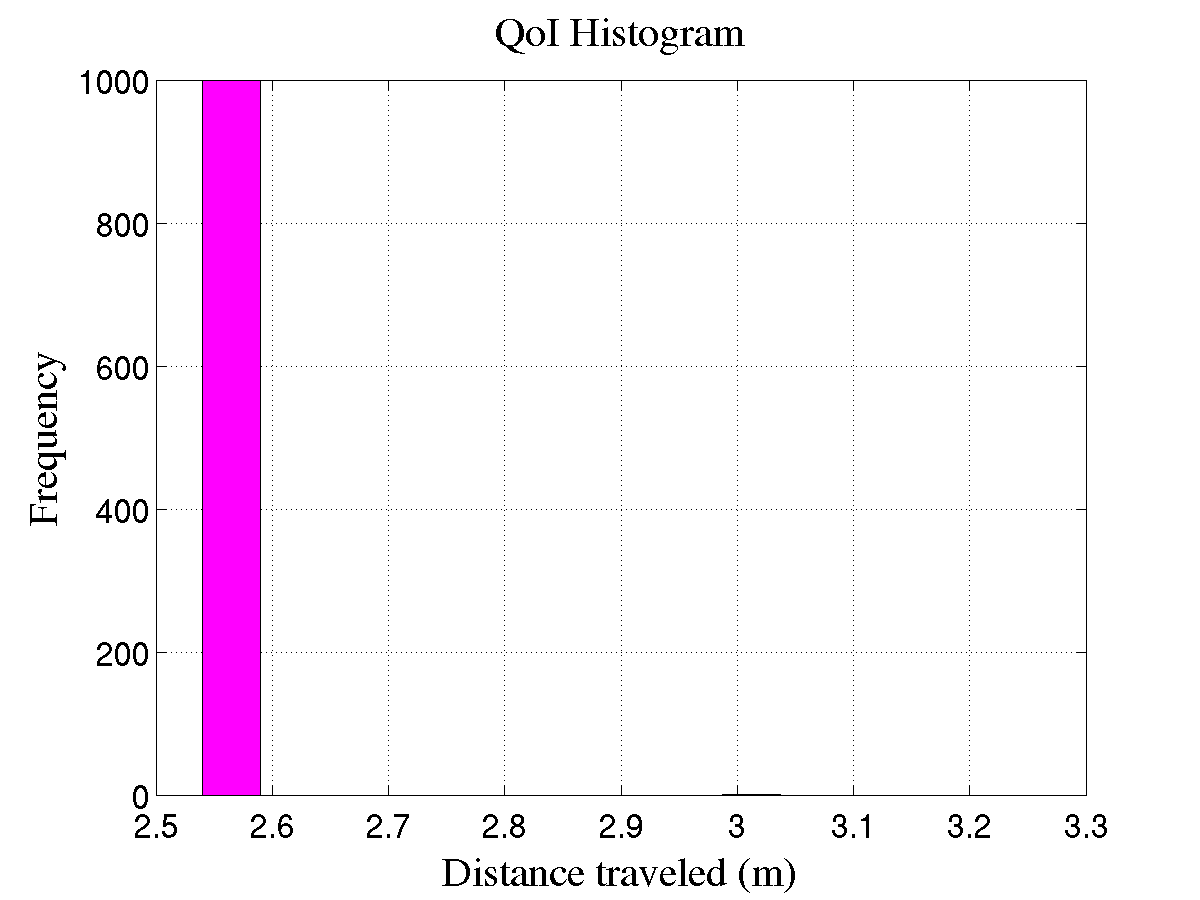
\includegraphics[scale=0.35]{figs/sfp_gravity_hist.png}\label{fig:sfp_gravity_hist}}
\vspace{-6pt}
\caption{MC chain positions and histogram of QoI $=d$.}
\end{figure}

\paragraph{KDE Plots} \

Matlab function \verb+ksdensity+ (Kernel smoothing density estimate) together with the option \verb+'pdf'+ may be used for plotting the KDE of the he QoI, displayed in Figure \ref{fig:sfp_gravity_kde}.

\begin{lstlisting}[label=matlab:kde_qoi,caption={Matlab code for the QoI KDE plot.}]
% inside Matlab
>> sfp_gravity_qoi_seq.m
>> [f,xi] = ksdensity(fp_mc_QoiSeq_unified,'function','pdf');
>> plot(xi,f,'-b','linewidth',3)
>> title('QoI Kernel Density Estimation ','fontsize',20);
>> xlabel('Distance traveled (m)','fontsize',20);
>> ylabel('KDE','fontsize',20);
>> grid on;
\end{lstlisting}

% \begin{figure}[htp]
% \centering 
% 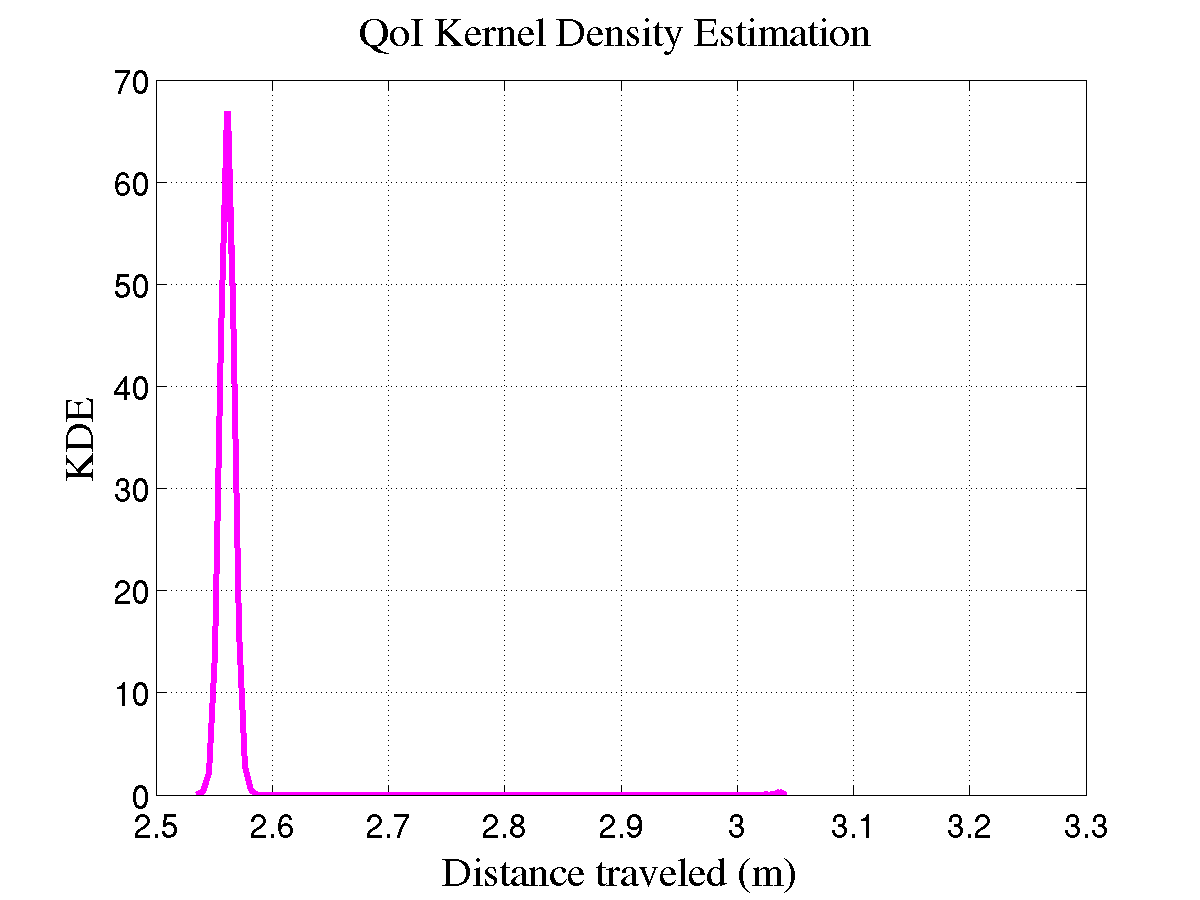
\includegraphics[scale=0.35]{figs/sfp_gravity_kde.png}
% \vspace*{-10pt}
% \caption{Kernel Density Estimation.}
% \label{fig:sfp_gravity_kde}
% \end{figure}

% \newpage

\paragraph{CDF Plots} \

Matlab function \verb+ksdensity+ (Kernel smoothing density estimate) with \verb+'cdf'+ option may also be used for plotting the Cumulative Distribution Function of the QoI, displayed in Figure~\ref{fig:sfp_gravity_cdf}.

\begin{lstlisting}[label=matlab:cdf_qoi,caption={Matlab code for the QoI CDF plot.}]
% inside Matlab
>> sfp_gravity_qoi_seq.m
>> [f,xi] = ksdensity(fp_mc_QoiSeq_unified,'function','cdf');
>> plot(xi,f,'-b','linewidth',3)
>> title('QoI Cumulative Distribution Function ','fontsize',20);
>> xlabel('Distance traveled (m)','fontsize',20);
>> ylabel('CDF','fontsize',20);
>> grid on;
\end{lstlisting}
% 
% \begin{figure}[p]
% \centering 
% 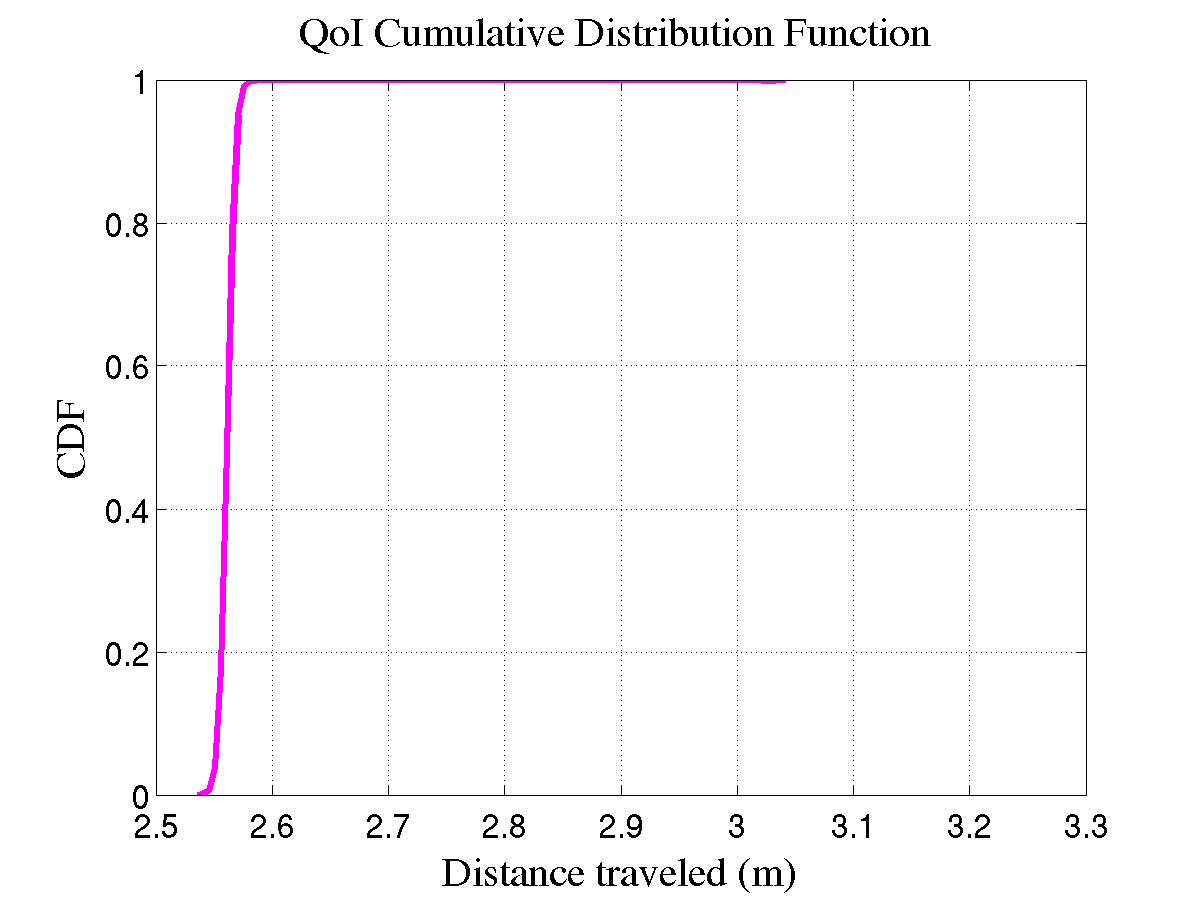
\includegraphics[scale=0.35]{figs/sfp_gravity_cdf.png}
% \vspace*{-10pt}
% \caption{Cumulative Distribution Function.}
% \label{fig:sfp_gravity_cdf}
% \end{figure}

\begin{figure}[htp]
\centering 
\subfloat[KDE]{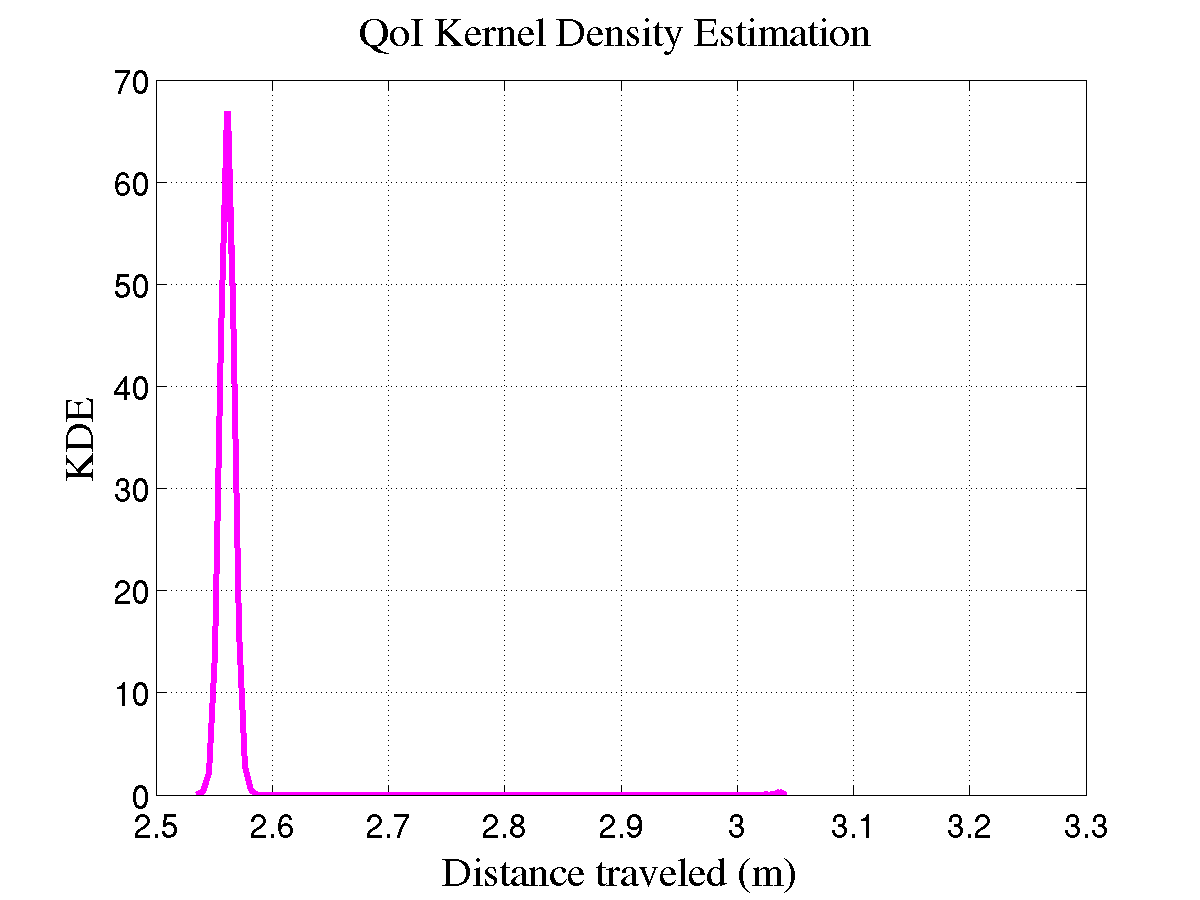
\includegraphics[scale=0.35]{figs/sfp_gravity_kde.png}\label{fig:sfp_gravity_kde}}
\subfloat[CDF]{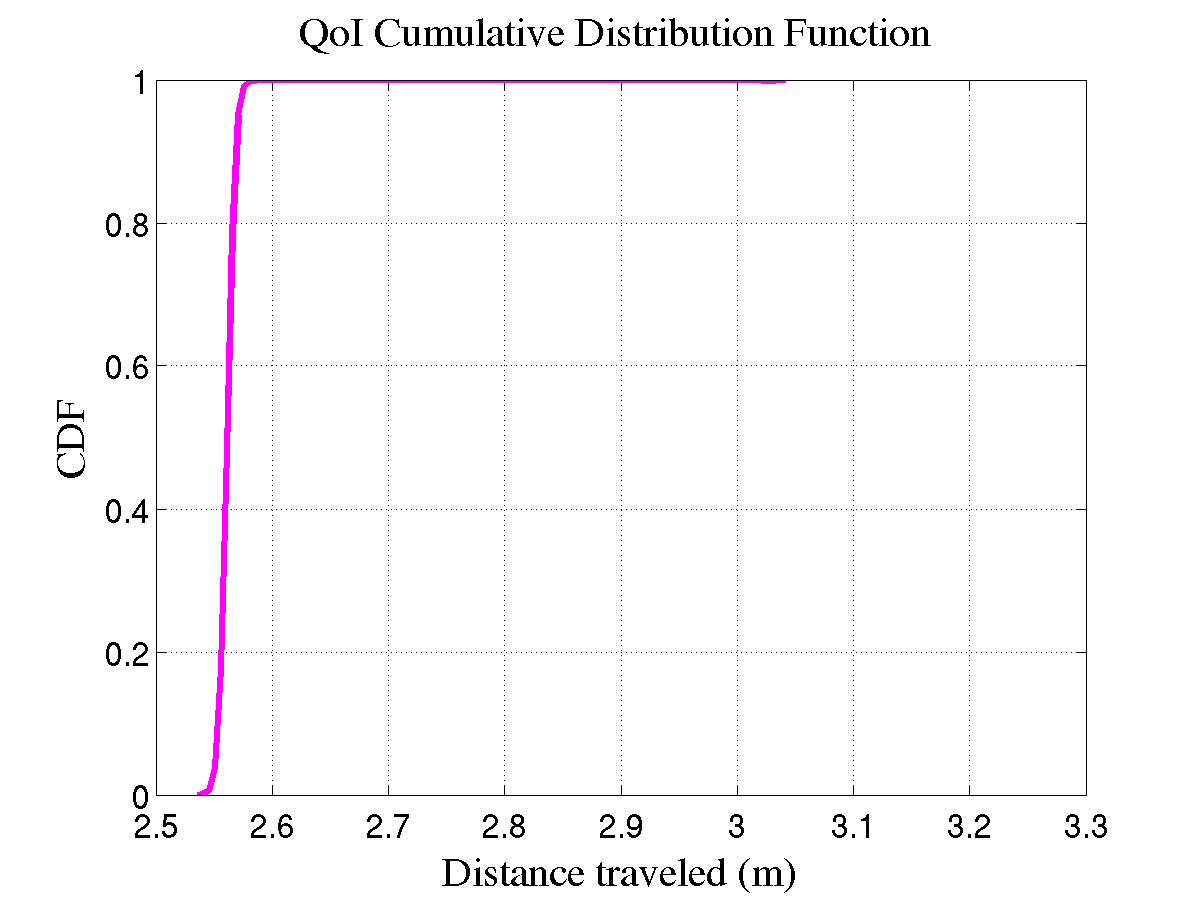
\includegraphics[scale=0.35]{figs/sfp_gravity_cdf.png}\label{fig:sfp_gravity_cdf}}
\vspace*{-6pt}
\caption{Kernel Density Estimation and Cumulative Distribution Function of QoI.}
\end{figure}
\paragraph{Autocorrelation Plots} \

The code presented in Listing \ref{matlab:autocorr_qoi} uses Matlab function \verb+autocorr+ to generate Figure~\ref{fig:sfp_gravity_autocorrelation}, which presents the autocorrelation of the QoI $d$.

\begin{lstlisting}[label=matlab:autocorr_qoi,caption={Matlab code for the QoI autocorrelation plot.}]
% inside Matlab
>> sfp_gravity_qoi_seq.m
>> nlags=10;
>> [ACF, lags, bounds] = autocorr(fp_mc_QoiSeq_unified, nlags, 0);
>> plot(lags,ACF,'bo-','linewidth',3);
>> ylabel('Autocorrelation for QoI = d','fontsize',20);
>> xlabel('Lag','fontsize',20);
>> title('QoI Autocorrelation','fontsize',20);
>> grid on;
\end{lstlisting}

\begin{figure}[htp]
\centering
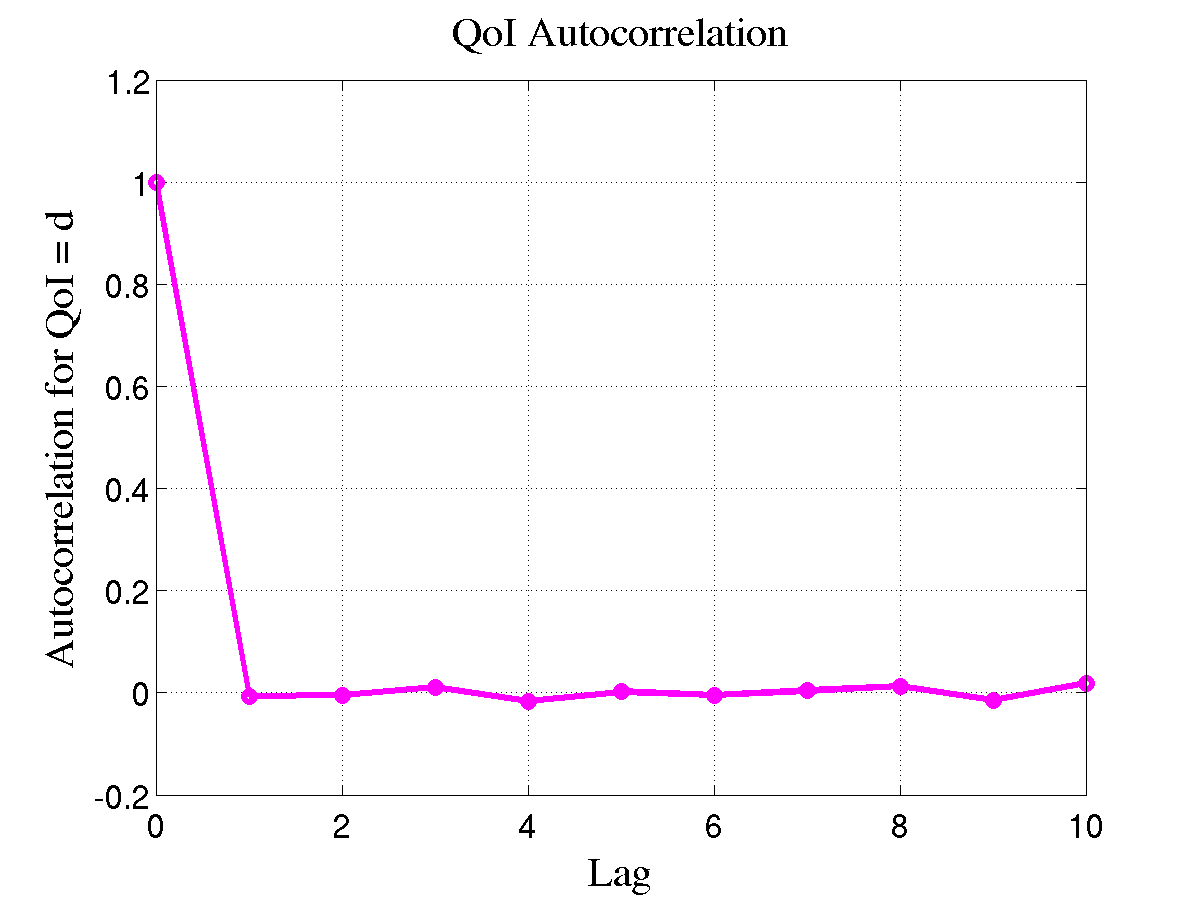
\includegraphics[scale=0.35]{figs/sfp_gravity_autocorrelation.png}
\vspace*{-10pt}
\caption{Autocorrelation plot.}
\label{fig:sfp_gravity_autocorrelation}
\end{figure}

\paragraph{Covariance and Correlation Matrices} \

For a matrix input \verb+X+, where each row is an observation, and each column is a variable, the Matlab function \verb+cov(X)+ may be used to calculate the covariance matrix.
%The command \verb+diag(cov(X))+ is a vector of variances for each column, and, therefore, \verb+sqrt(diag(cov(X)))+ is a vector of standard deviations.  

Thus,  in order to calculated the covariance matrix between the parameter and the quantity of interest sequences generated by Monte Carlo sampler with QUESO,
one may simply define \verb+X=[fp_mc_ParamSeq_unified fp_mc_QoiSeq_unified]+.
The code presented in Listing \ref{matlab:cov_pqoi} shows the usage of Matlab commands for finding such the matrix.

\begin{lstlisting}[label=matlab:cov_pqoi,caption={Matlab code for the matrix of covariance between parameter $g$ and QoI $d$.}]
% inside Matlab
>> sfp_gravity_qoi_seq;
>> sfp_gravity_p_seq;
>> X=[fp_mc_ParamSeq_unified fp_mc_QoiSeq_unified];
>> cov_p_QoI = cov(X)

cov_p_QoI =
	  [ 2.826e-03 	-8.555e-04 ] 
	  [-8.555e-04 	 2.599e-04 ]

\end{lstlisting}

Analogously, the Matlab function \verb+corrcoef(X)+ returns a matrix of correlation coefficients calculated from an input matrix \verb+X+ whose rows are observations and whose columns are variables.
In order to calculated the correlation matrix between the parameter and the QoI sequences, one may simply define \verb+X=[fp_mc_ParamSeq_unified fp_mc_QoiSeq_unified]+.
% The matrix R = corrcoef(X) is related to the covariance matrix C = cov(X) b

\begin{lstlisting}[label=matlab:corr_param_qoi,caption={Matlab code for the matrix of correlation between parameter $g$ and quantity of interest $d$.}]
% inside Matlab
>> sfp_gravity_qoi_seq;
>> sfp_gravity_p_seq;
>> X=[fp_mc_ParamSeq_unified fp_mc_QoiSeq_unified];
>> corr_p_QoI = corrcoef(X)

corr_p_QoI =
	  [ 1.000e+00 	-9.981e-01 ] 
	  [-9.981e-01 	 1.000e+00 ]
>>
\end{lstlisting}


